\section{Planificación del Trabajo}

\subsection{Descripción del grupo de trabajo}

\subsection{Estimación de esfuerzo}
Hemos analizado todos los aspectos posibles que serán parte del desarrollo de nuestro software y que competen a la estimación de esfuerzo, sin embargo, todo lo analizado queda sujeto a modificaciones, debido principalmente a que el proyecto está aún en desarrollo y no poseemos una base o una visión clara del producto final. Tanto a nivel de programación como de diseño a de ser necesaria una frecuente revisión y actualización con cada iteración y avance en este proyecto.

Según lo conversado, pactado y analizado con mis compañeros de trabajo en la primera iteración, los análisis del proyecto se puede apreciar en las siguientes graficas de estimación de puntos de esfuerzo.
\begin{figure}[htbp]
	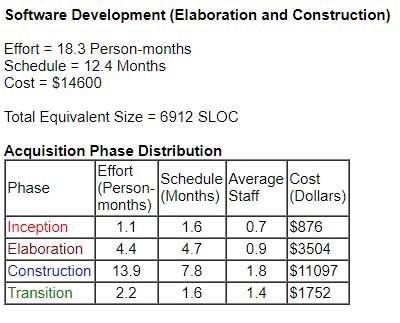
\includegraphics{1.JPG}
	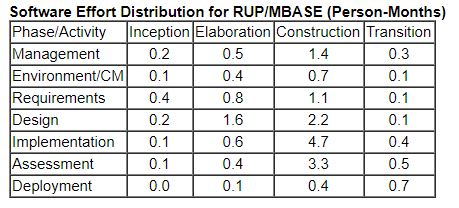
\includegraphics[scale=0.9]{2.JPG}
\end{figure}

\begin{figure}[htbp]
	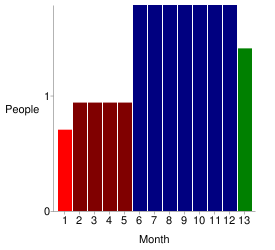
\includegraphics{Grafica.png}
	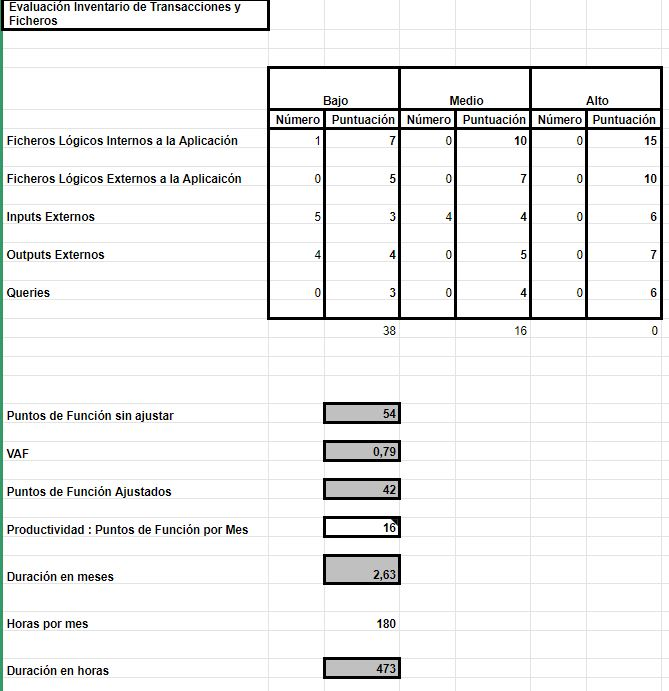
\includegraphics[scale=0.5]{Estimacion de PF.JPG}
\end{figure}

\subsection{Asignación de recursos}

\subsection{Planificación temporal de actividades}